\section{Future Work}
\label{cp7:future-work}



In this section, we elaborate some of the future research  
mentioned in Sections~\ref{cp7:relevance} and~\ref{cp7:deployment}.
We also discuss other avenues for future work.


\subsection{Relevance Datasets}
\label{cp7:gauging}


In Section~\ref{cp7:relevance}, we indicated that future studies should further investigate 
what kind of information developers deem relevant and how developers gauge relevance.
Upon reflecting on the data-gathering procedures described throughout this work,
a potential line of work is to consider 
gathering data from software professionals performing daily tasks in a non-obstructive way.



Conducting empirical
 experiments in a more realistic environment is challenging~\cite{Kevic2015}.
This effort is worthwhile as
the richness of collected data can provide valuable insights
to provide a foundation for tool development.
One potential method for
data collection 
considers 
how recent studies with eye-trackers~\cite{Cutrell2007, Petrusel2013, sharafi2020}
have shown that the technology is not as disruptive as other 
methods~\cite{Lazar2017} such as think aloud protocols or manual input. 
Hence, we believe that eye-tracking 
could be used in a developer's working environment, 
leading to more realistic data on which text developers perceive as task-relevant.
For example, one could
extend the work done by Kevic and colleagues on
tracing developers' eye for change tasks~\cite{Kevic2015} to
also consider tracing data outside a developer's IDE
for such a purpose.



A second venue is to consider who perceived which text as relevant.
As observed both in related work~\cite{Crosby1990, Busjahn2015} and in our formative study (Chapter~\ref{ch:characterizing}),
there is variability in what text may be relevant to a software task and 
providing more background data about 
the participants who considered some information useful could lead to benchmarks 
for evaluating techniques
focused on a certain population (e.g., expert versus novice developers~\cite{Crosby1990, Busjahn2015}). 



% In Chapter~\ref{ch:related-work}, we described 
% a series of studies that mine text from natural language artifacts.
% These studies provide annotated data 
% resulting from coding procedures that usually do not take into account
% differences in what might be relevant; or disagreements are resolved during the annotation process. 
% However, in our formative study (Chapter~\ref{ch:characterizing}),
% we have observed that there is variability in what text may be relevant 
% to a software task, a fact that other researchers have also brought to light~\cite{Bavota2016,Robillard2015}.









\subsection{Sentence Semantics}
\label{cp7:semantics}




In Chapter~\ref{ch:characterizing}, we used frame semantics, a general linguistic approach~\cite{fillmore1976frame},
as a means for access to the meaning of the text in natural language software artifacts.
However, questions remain about whether
semantic frames can help in identifying the semantics of software engineering text
and the extent to which it applies to software engineering text.




We partially addressed these questions in a study, 
orthogonal to this dissertation~\cite{marques2021},
where we assess the applicability of generic semantic frame
parsing to software engineering text
aimed at supporting program
comprehension activities.
In this study, we first assessed how the tool we used in Chapter~\ref{ch:characterizing}
to analyze the meaning of the text considered relevant (i.e., SEMAFOR~\cite{das2014frame})
 applies to text sampled from 1,802 documents drawn from a set of datasets~\cite{Arya2019, Xu2017, Maalej2013, Chaparro2017}. 
Based on the results from this analysis, 
we proposed \textit{SEFrame}, a tool that tailors 
frame parsing to natural language text in software engineering artifacts.
Results from a second evaluation indicated that \textit{SEFrame} was 
 correct in between 73\% and 74\% of
the cases and that it parsed text from a variety of software artifacts used to support program
comprehension, which motivated our decision to apply \textit{SEFrame} 
in the design of the techniques we explored in Chapter~\ref{ch:identifying}.


Future research should consider
a more in depth investigation of 
frame semantics or other general approaches that can infer the meaning of text at the sentence level. 
For example, future studies could focus on answering 
which frames most accurately capture the information conveyed in the text 
and how frames extracted by state-of-the-art tools (e.g.,~\cite{swayamdipta17, chen2021joint})
compare to manual labels provided by researchers 
about the information available in certain kinds of software artifacts~\cite{Maalej2013, Arya2019, Sorbo2015}.  



 






\subsection{Deep Learning for Software Engineering}
\label{cp7:deep-learning}



Future research in the field of deep learning for software engineering could consider 
exploring other pre-trained \acs{DL} models as well as other applications of 
deep-learning to software engineering tasks. 




In Chapter~\ref{ch:identifying}, we have discussed threats associated with the BERT pre-trained model 
we used and how future research should consider other 
general or software-specific pre-trained models.
We did not explore other general pre-trained models because most of the models that apply to our domain problem 
are variations of BERT (e.g., Albert~\cite{lan2019albert} or Roberta~\cite{liu2019roberta})
and by using the BERT base model, we sought to establish a baseline for future comparisons.




With regards to software-specific models (e.g., ~\cite{feng2020-codebert, li2019neural}), we also emphasize 
that these models have been trained on either source code or source code and method level text documentation. 
These datasets might not align with how developers discuss text in natural language artifacts~\cite{arya2020}, such 
as Stack Overflow posts or web tutorials. Therefore, future research should consider how 
 models pre-trained on text originating from various kinds of 
natural language software artifacts compare to the base model that we used.





In Chapter~\ref{ch:identifying}, we have shown that artifact-specific techniques, such as AnswerBot, have accuracy comparable to the semantic-based approaches
we have explored. This  provides
a unique opportunity for the creation of synthetic data that we can use to further fine-tune the deep-learning models we explored.
For that, future research should show that models trained on synthetic data
 extend beyond what an artifact-specific technique used for bootstrapping already provides. For example, showing that
a model fine-tuned using synthetic data can identify task-relevant textual information in a different type of artifact or showing
that the model's accuracy is significantly better than the technique used for bootstrapping.


% \art{Think whether I need anything else in this section}


% As  other potential applications of \acs{DL}, we highlight how researchers can use BERT's attention mechanism~\cite{Vaswani2017attention}
% in software engineering activities such as finding who should fix a bug~\cite{anvik2006}, requirements traceability~\cite{Lin2021}


% in sentence pairs. As we have described in Section~\ref{cp5:approach-bert}, we used this mechanism to correlate the text in natural language artifacts and the text in a task and future research could explore applying attention for recommending  
% or in other words pairing the text in 
% or 








\subsection{Presenting Task-Relevant Text}
\label{cp7:info-viz}




In Chapter~\ref{ch:assisting}, we described how \acs{tool}
highlights the text in a natural language artifact that it identifies 
as relevant to an input task. Our idea to highlight text 
draws from related work which suggests that textual highlights 
are a simple approach to surface the most important information in 
an artifact~\cite{Robillard2015,nadi2020}. 
Although simple, participants shared limitations of 
this strategy:



\smallskip
\begin{quote}
``\textit{It was much easier to follow with previously highlighted text.  
    However, it would have been nicer to have some sort of side bar/index of highlighted snippets
    where I could know and scroll directly through the highlighted parts of a page.}''---P9
\end{quote}



\smallskip
\begin{quote}
``\textit{There was a resource page which was super long, and I found it very difficult to locate which sentences were highlighted, therefore, making that resource useless to me because I didn't have the motivation to scroll through it to find all highlights. An interface that gathers highlight locations would make a difference.}''---P21
\end{quote}


\smallskip
This feedback made us question other potential ways to present the text identified by \acs{tool}.
For example, we could have followed design principles adopted by Unakite~\cite{Liu2018Unakite}---a tool that collects, organizes and keeps track of information---to make \acs{tool} display the text identified on its context menu.
Figure~\ref{fig:navigational-cues} shows a mock up of \acs{tool} bundling the highlights identified for one of the artifacts in the \texttt{titanic} task (Section~\ref{cp6:tasks}).
Using this context menu, a user could click on the text identified and navigate to the part of the documentation 
originally containing the text.



\begin{figure}[H]
    \centering
    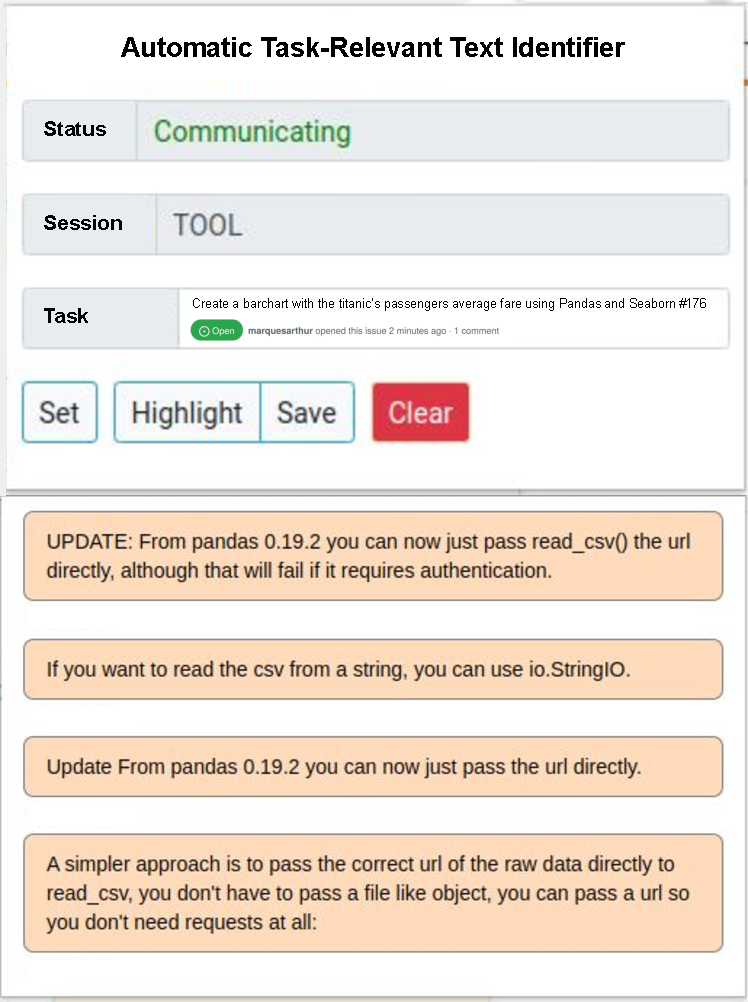
\includegraphics[width=0.55\textwidth]{fig/cp7/navigational-cues}
    \caption{Mock up of the highlights identified by \acs{tool} as navigational cues; by clicking on a highlight, a user could be directed to the part of a document containing that highlight}
    \label{fig:navigational-cues}
\end{figure}



A second approach to organizing the text identified could consider 
the semantic meaning of each sentence, as extracted through frame semantics or other semantic-based approaches. 
Semantic frames could 
assist a user in comprehending the content of the text automatically identified
without the need to read it. 
As done by Libra~\cite{Ponzanelli2017}, semantic frames could also be used to group the text identified in bubbles or a hierarchical representation 
 helping a developer
in deciding what portions of the text they would inspect first. 
Figure~\ref{fig:semantic-cues} shows a mock up 
with some of the semantic frames extracted 
for the sentences in Figure~\ref{fig:navigational-cues}.
Using the semantic frames identified,
a developer could decide whether they would read sentences 
describing some coding procedure (\textit{execution}), or sentences 
with warnings or requirements about the Pandas API (\textit{requirement} and \textit{being obligated}). 
To be useful, future research must consider how to identify from all the frames available in a sentence, 
which frames
better summarize the meaning of the text. 


We leave the investigation of other ways to present task-relevant text to future research.




\begin{figure}
    \centering
    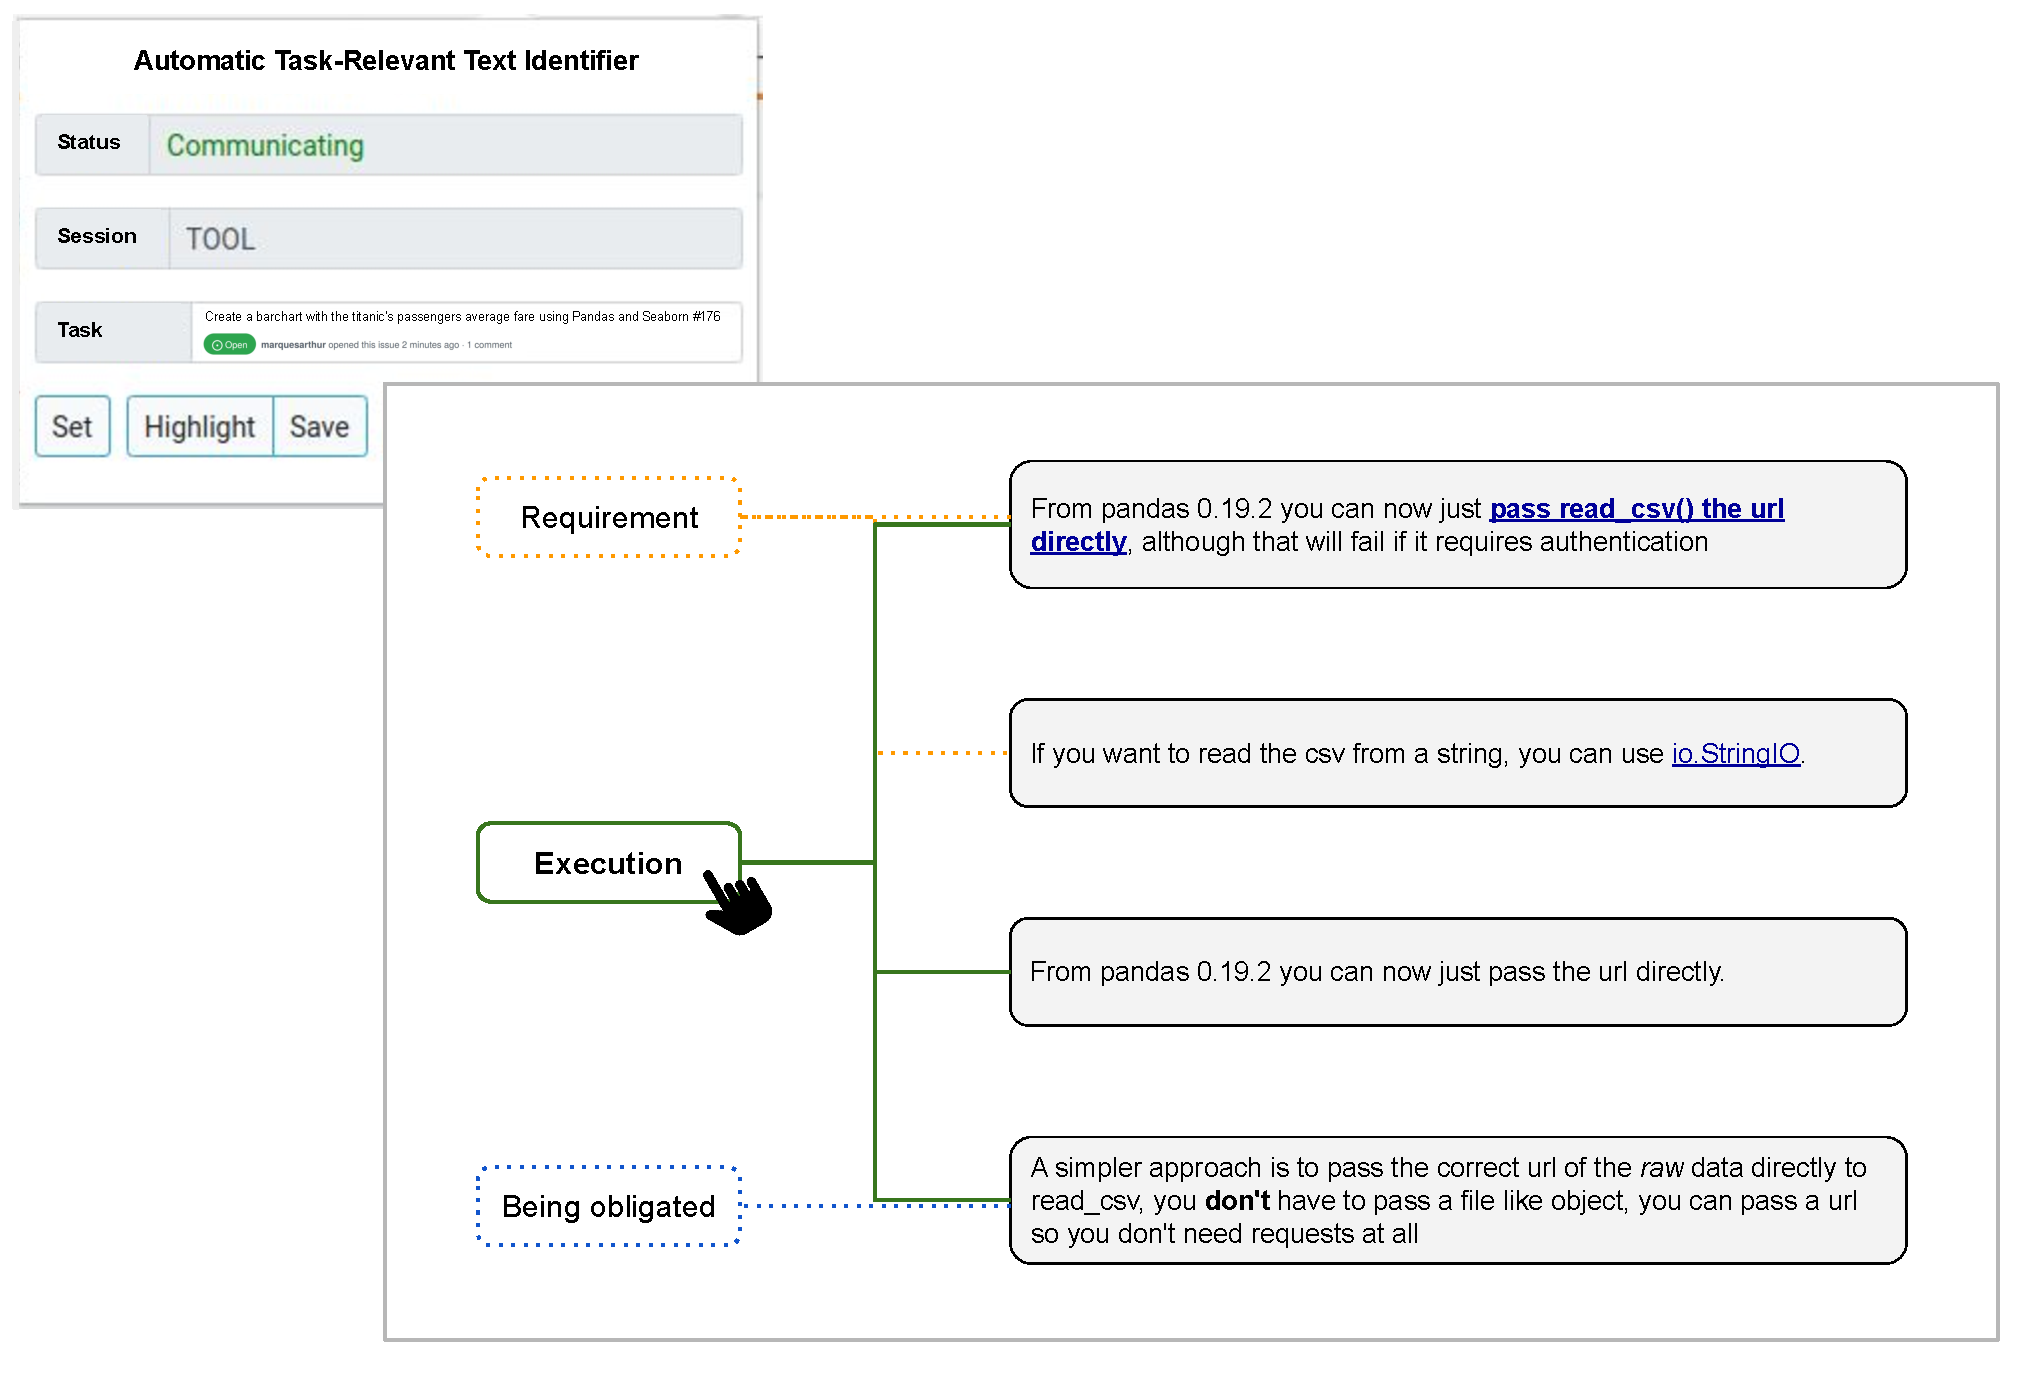
\includegraphics[width=0.90\textwidth]{fig/cp7/semantic-cues}
    \caption{Mock up of the highlights grouped by semantic frames; by hovering over a semantic frame, a user could quickly identify which of the text identified is associated with a certain meaning}
    \label{fig:semantic-cues}
\end{figure}





